\section{An improved Metropolis-Hasting algorithm}
%\vspace{-.05in}
The algorithm we propose symmetrizes the probability of $W$ under the old and new parameters, so that $P(W|\theta)$ disappears from the acceptance ratio. 
Now, the probability of accepting a proposal $\vartheta$ will depend only on the prior probabilities of $\theta$ and $\vartheta$, as well as how well they both explain the data given $W$.
This is in contrast to the previous algorithm, where one must also factor in how well each parameter explains the current value of the grid $W$.
This results in a MCMC sampler that mixes significantly more rapidly. 
Since we need not account for the probabilities $P(W|\theta)$, we also have a simpler MCMC scheme.
%This forms the main contribution of this paper.

As before, the MCMC iteration begins with $(s_0, S, T, \theta)$. 
Instead of simulating the thinned events $U$ like earlier algorithms, we {\em first} generate a new parameter $\vartheta$ from some distribution $q(\vartheta|\theta)$. 
Treat this as an auxiliary variable, so that the augmented space now is $(s_0,S, T, \theta,\vartheta)$. 
Define a function $\Omega(\theta,\vartheta) > \max_s A_s(\theta)$ that is symmetric in its arguments (the number of arguments will distinguish $\Omega(\cdot,\cdot)$ from $\Omega(\cdot)$ of the earlier sections).
Two examples are $\Omega(\theta,\vartheta) = \kappa \max_s A_s(\theta) + \kappa \max_s A_s(\vartheta)$, for $\kappa \ge 1$, and 
$\Omega(\theta,\vartheta) = \kappa \max\left(\max_s A_s(\theta), \max_s A_s(\vartheta)\right)$, for $\kappa > 1$.


We will treat the path $(s_0,S,T)$ as simulated by  uniformization, but now with the dominating Poisson rate equal to $\Omega(\theta,\vartheta)$  instead of $\Omega(\theta)$. 
The transition matrix $B(\theta,\vartheta)$ of the embedded Markov chain is $B(\theta,\vartheta) = I + \frac{1}{\Omega(\theta,\vartheta)}A(\theta)$, so that the resulting trajectory $(s_0,S,T)$ will still be a realization from a MJP with rate-matrix $A(\theta)$.

Following the Rao-Teh algorithm, the conditional distribution of the thinned events $U$ given $(s_0,S,T,\theta,\vartheta)$ is a piecewise-constant Poisson with rate $\Omega(\theta, \vartheta) - A_{S(t)}(\theta), t \in [0,t_{end})$. 
This reconstructs the set $W = U \cup T$,  and as we saw~\citep[see also][]{RaoTeh13}, $P(W|\theta,\vartheta)$ is a homogeneous Poisson process with rate $\Omega(\theta, \vartheta)$. 
%which, crucially, is symmetric in $\theta$ and $\vartheta$. 
Having imputed $W$, discard the state values, so that the MCMC state space is $(W, \theta, \vartheta)$.
Now, propose swapping $\theta$ with $\vartheta$. 
From the symmetry of $\Omega(\cdot,\cdot)$, the Poisson grid $W$ has the same probability both
before and after this proposal, so unlike the previous scheme, the ratio %$P(W|\vartheta)/P(W|\theta)$ 
equals $1$.  
This simplifies computation, and as suggested in the previous section, can significantly improve mixing.
An acceptance probability of
$ 
% \min\left(1, \frac{P(X,\vartheta)q(\theta|\vartheta)}
%  {P(X,\theta)q(\vartheta|\theta)}\right) = 
  \min\left(1, \frac{P(X|W,\vartheta,\theta) P(\vartheta) q(\theta|\vartheta)}
   {P(X|W,\theta,\vartheta) P(\theta)q(\vartheta|\theta)}\right)
   $ 
   targets the conditional $P(W,\theta,\vartheta|X) \propto P(\theta)q(\vartheta|\theta)P(W,X|\theta,\vartheta)$.
   The terms $P(X|\vartheta)$ and  $P(X|\theta)$ can be calculated from the forward pass of FFBS, and after
   accepting or rejecting the proposal, a new trajectory is sampled by
   completing the backward pass. Finally, the thinned events and auxiliary parameter are
   discarded. Algorithm~\ref{alg:MH_improved} and 
   figure~\ref{fig:MH_improved} outline the details of these steps. 
\begin{algorithm}[H]
   \caption{Symmetrized MH for parameter inference for MJPs }
   \label{alg:MH_improved}
  \begin{tabular}{l l}
   \textbf{Input:  } & \text{The observations $X$,}
                      \text{the MJP path $(s_0, S, T)$, MJP parameters $\theta$} and $\pi_0$.\\ 
   %                & \text{A  Metropolis-Hasting proposal $q(\cdot | \theta)$}.\\
   \textbf{Output:  }& \text{A new MJP trajectory $(s'_0, S', T')$, 
                            new MJP parameters $\theta'$}.\\
   \hline
   \end{tabular}
   \begin{algorithmic}[1]
     \State \textbf{Sample $\vartheta \sim q(\cdot| \theta)$}, and 
      set %$\Omega = \max_i A_i(\theta) + \max_i A_i(\theta^*)$. 
	$\Omega \assign \Omega(\theta,\vartheta)$ % + \Omega(\vartheta)$ 
    for some symmetric $\Omega(\theta,\vartheta) > \max_s A_s(\theta)$.
      %In the case of uniformization, we
      %have a single $\Omega$ for all states, with $\Omega = \max_i A_i(\theta) + \max_i A_i(\theta^*)$.
      %, with $h(\theta) > max_s{|A_s(\theta)|}$, $h(\theta^*) > max_s{|A_s(\theta^*)|}$ using some deterministic function $h$.
    \State \textbf{Simulate the thinned times $U$} from a rate-$(\Omega-A_{S(\cdot)}(\theta))$ Poisson process:

    \vspace{-.05in}
    $\qquad \qquad \qquad \qquad U \sim \text{PoissProc}(\Omega - A_{S(t)}(\theta)), \quad t \in [0,t_{end})$.
    \State Set $W = T \cup U$ and discard $(s_0,S)$. Define $\tilde{W} = 0 \cup W \cup t_{end}$.
%    \State Set $W = T \cup U$ and discard MJP states $S$. The MCMC state is now $(\theta,\vartheta, W)$.
 %   \State \textbf{MH proposal}: The current MCMC state-space is $(W,\theta,\vartheta)$. 
 %   Propose swapping $\theta$ and $\vartheta$, so the new state-space is $(W,\vartheta,\theta)$. 
 %    Accept with probability 
 %    $ \text{acc} 
 %      =  1 \wedge \frac{P(X| W,\vartheta,\theta)P(\vartheta)q(\theta|\vartheta)}
 %      {P(X| W,\theta, \vartheta)P(\theta) q(\vartheta|\theta)}.
 %      $
    \State \textbf{Forward pass:} Set $B(\theta,\vartheta) = I + \frac{A(\theta)}{\Omega(\theta, \vartheta)}$ and $\fwd^{\theta, \vartheta}_0(\cdot) = \pi_0$. Recall $\ell_i(\cdot)$ from equation~\eqref{eq:lik_factor}.
    %Sequentially update $\fwd^{\theta,\vartheta}_i(\cdot)$ at $w_i \in W$ as: 
    \vspace{-.25in}
        $$\textbf{for } i=1\rightarrow |{W}|\textbf{ do:} \quad \fwd^{\theta,\vartheta}_i(s') = \sum_{s \in \cS} \fwd^{\theta,\vartheta}_{i-1}(s)\cdot \ell_{i}(s) \cdot B_{ss'}(\theta,\vartheta), \quad \forall s' \in \cS.\qquad\qquad\quad
    \vspace{-.1in}
        $$
        Similarly, for $B(\vartheta,\theta) = I + \frac{A(\vartheta)}{\Omega(\vartheta, \theta)}$, calculate $\fwd^{\vartheta,\theta}_i(\cdot)$ for all elements of ${W}$.
    \State \textbf{Swap} 
    $(\theta, \vartheta)$ with probability
     $
   %  \texttt{acc} =  
     1 \wedge \frac{P(X| W,\vartheta,\theta)P(\vartheta)q(\theta|\vartheta)}
        {P(X| W,\theta, \vartheta)P(\theta) q(\vartheta|\theta)}.
        $
    Write the new parameters as $(\theta',\vartheta')$.
        Here $P(X|W,\theta,\vartheta) = \sum_{s \in \cS} \fwd^{\theta,\vartheta}_{|W|}(s)\ell_{|W|+1}(s)$, $P(X|W,\vartheta,\theta) = \sum_{s \in \cS} \fwd^{\vartheta,\theta}_{|W|}(s)\ell_{|W|+1}(s)$.
    \State \textbf{Backward pass:}
    Simulate $v_{|W|} \sim \bck^{\theta',\vartheta'}_{|W|}(\cdot)$, where $\bck^{\theta',\vartheta'}_{|W|}\!(s) \propto \fwd^{\theta',\vartheta'}_{|W|}\!(s)\cdot\ell_{|W|+1}(s) \ \  \forall s \in \cS.$ 
    \vspace{-.25in}
    %For the new transition matrix $B(\theta',\vartheta')$,     
    $$\hspace{-.15in} \textbf{for } i=(|W|-1)\rightarrow 0\textbf{ do:} \ v_i \sim \bck^{\theta',\vartheta'}_i\!(\cdot), \text{where } 
    \bck^{\theta',\vartheta'}_i\!(s) \propto \fwd^{\theta',\vartheta'}_i\!(s)\cdot B_{sv_{i+1}}(\theta',\vartheta') \cdot \ell_{i+1}(s)  \ \forall s \in \cS.$$
    
%    Sample a path $\tilde{V}$, from a discret-time Markov chain with $|W| + 1$ steps, using FFBS algorithm. The transition matrix of the Markov chain is $B = (I + \frac{A(\tilde{\theta})}{\Omega})$ while the initial distribution over states is $\pi_0$. The likelihood of state $s$ at step $i$ is 
%    $$ L_i(s) = P(Y_{[w_i, w_{i + 1})} | S(t) = s \; for\; t \in [w_i, w_{i + 1})) = \prod_{j: t_j \in [w_i, w_{i + 1})}p(y_{t_j} | S(t_j) = s).$$\\
%%(i.e. $V(i) \sim P(V |  \theta(i), W(i - 1), y).$) Then delete all the virtual jumps to get $S(i), T(i) .$\\
    \vspace{-.1in}
    \State Set $s'_0=v_0$. Let $T'$ be the set of times in $W$ when $V$ changes state. Define $S'$ as the corresponding set of state values. Return $(s'_0, S', T', \theta')$.
\end{algorithmic}
\end{algorithm}

\setlength{\unitlength}{0.8cm}
  \begin{figure}[h!]
  \centering
  \begin{minipage}[!hp]{0.32\linewidth}
  \centering
    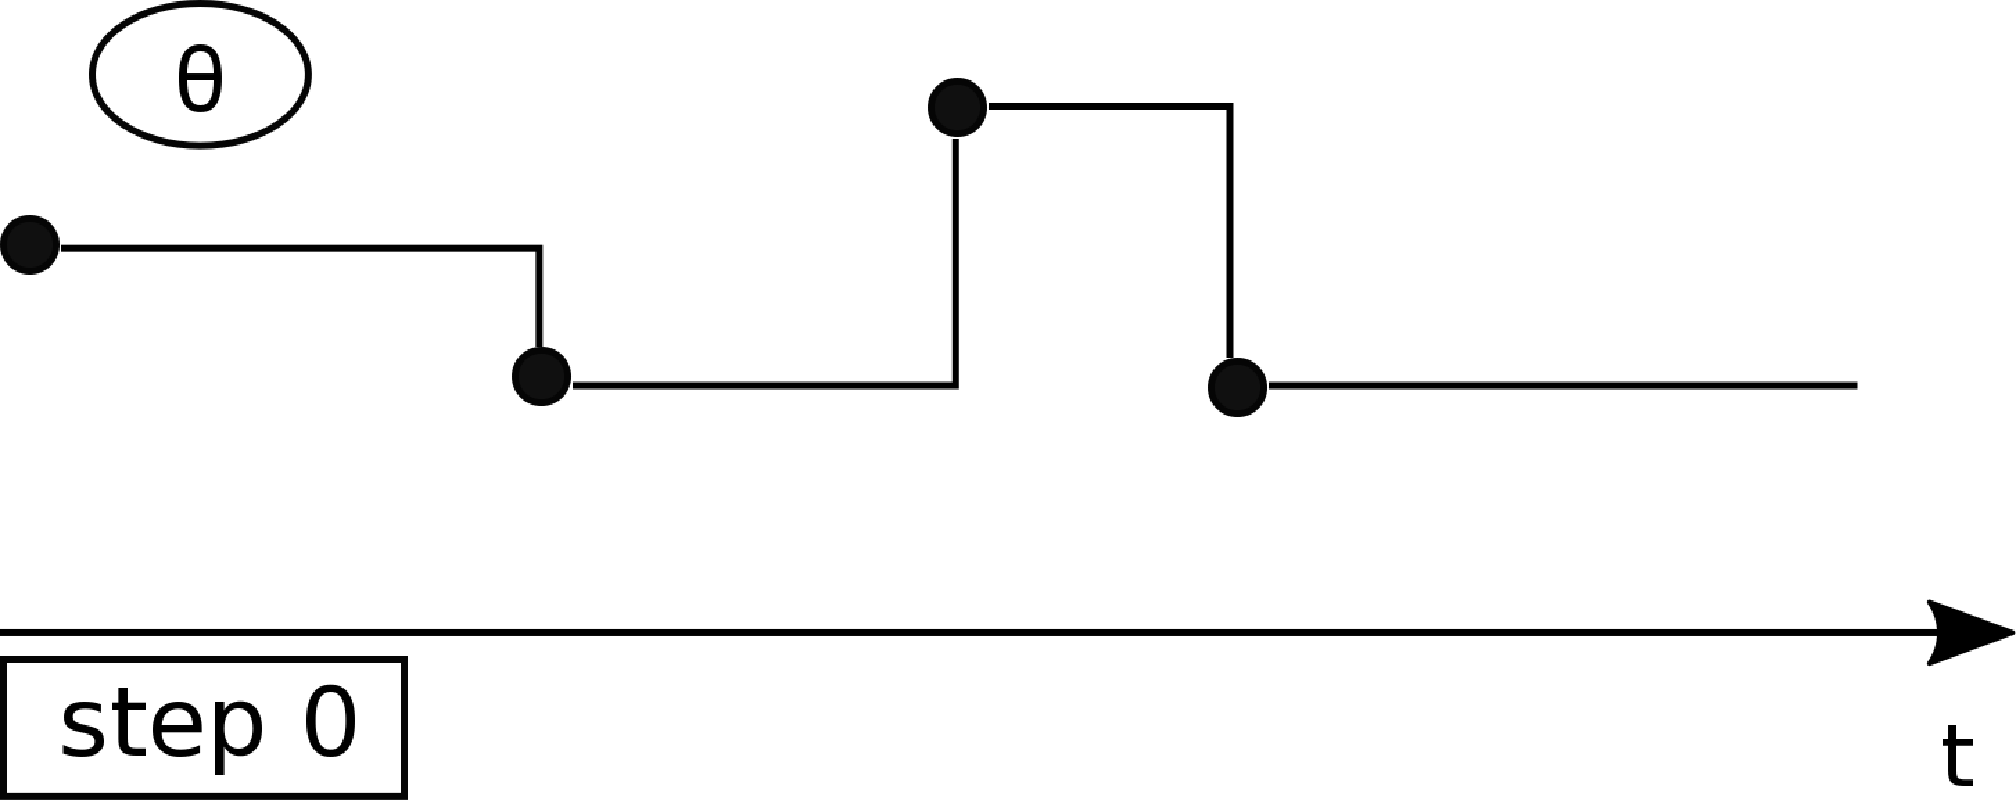
\includegraphics [width=0.96\textwidth, angle=0]{figs/plot0.png}
      \end{minipage}
  \begin{minipage}[hp]{0.32\linewidth}
  \centering
    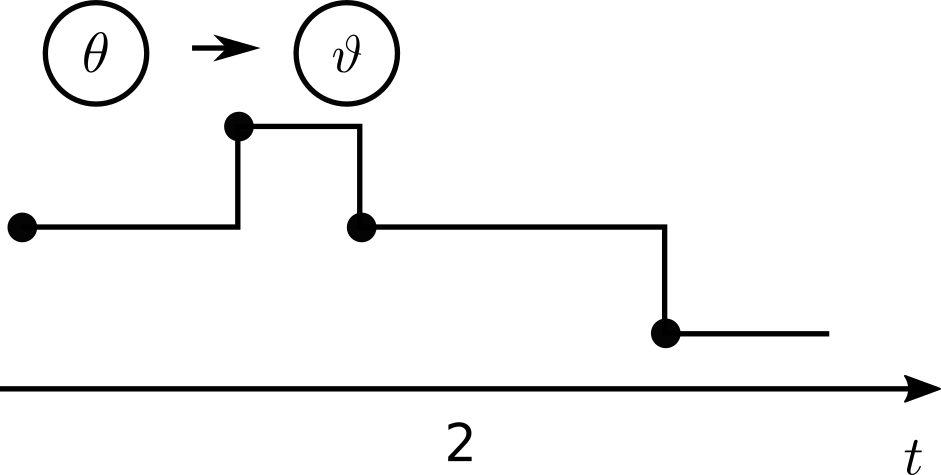
\includegraphics [width=0.96\textwidth, angle=0]{figs/plot1.png}
    \vspace{-0 in}
  \end{minipage}
  \begin{minipage}[hp]{0.32\linewidth}
  \centering
    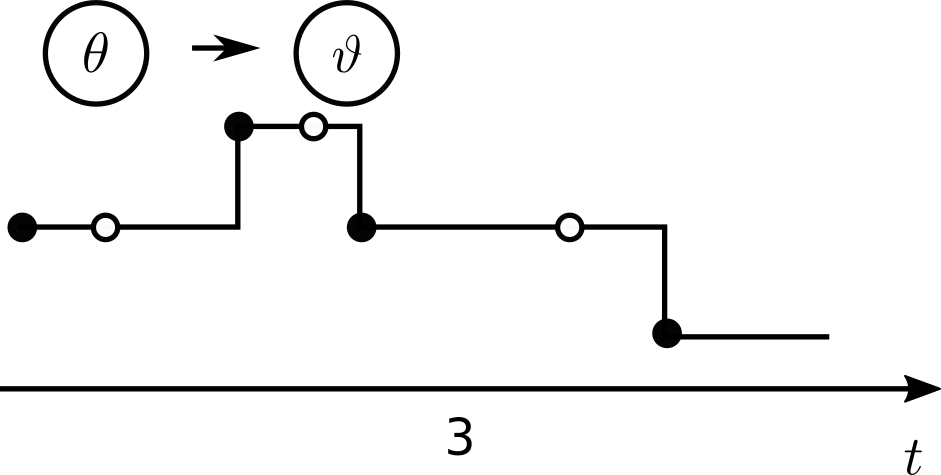
\includegraphics [width=0.96\textwidth, angle=0]{figs/plot2.png}
    \vspace{-0 in}
  \end{minipage}
  \begin{minipage}[hp]{0.32\linewidth}
  \centering
    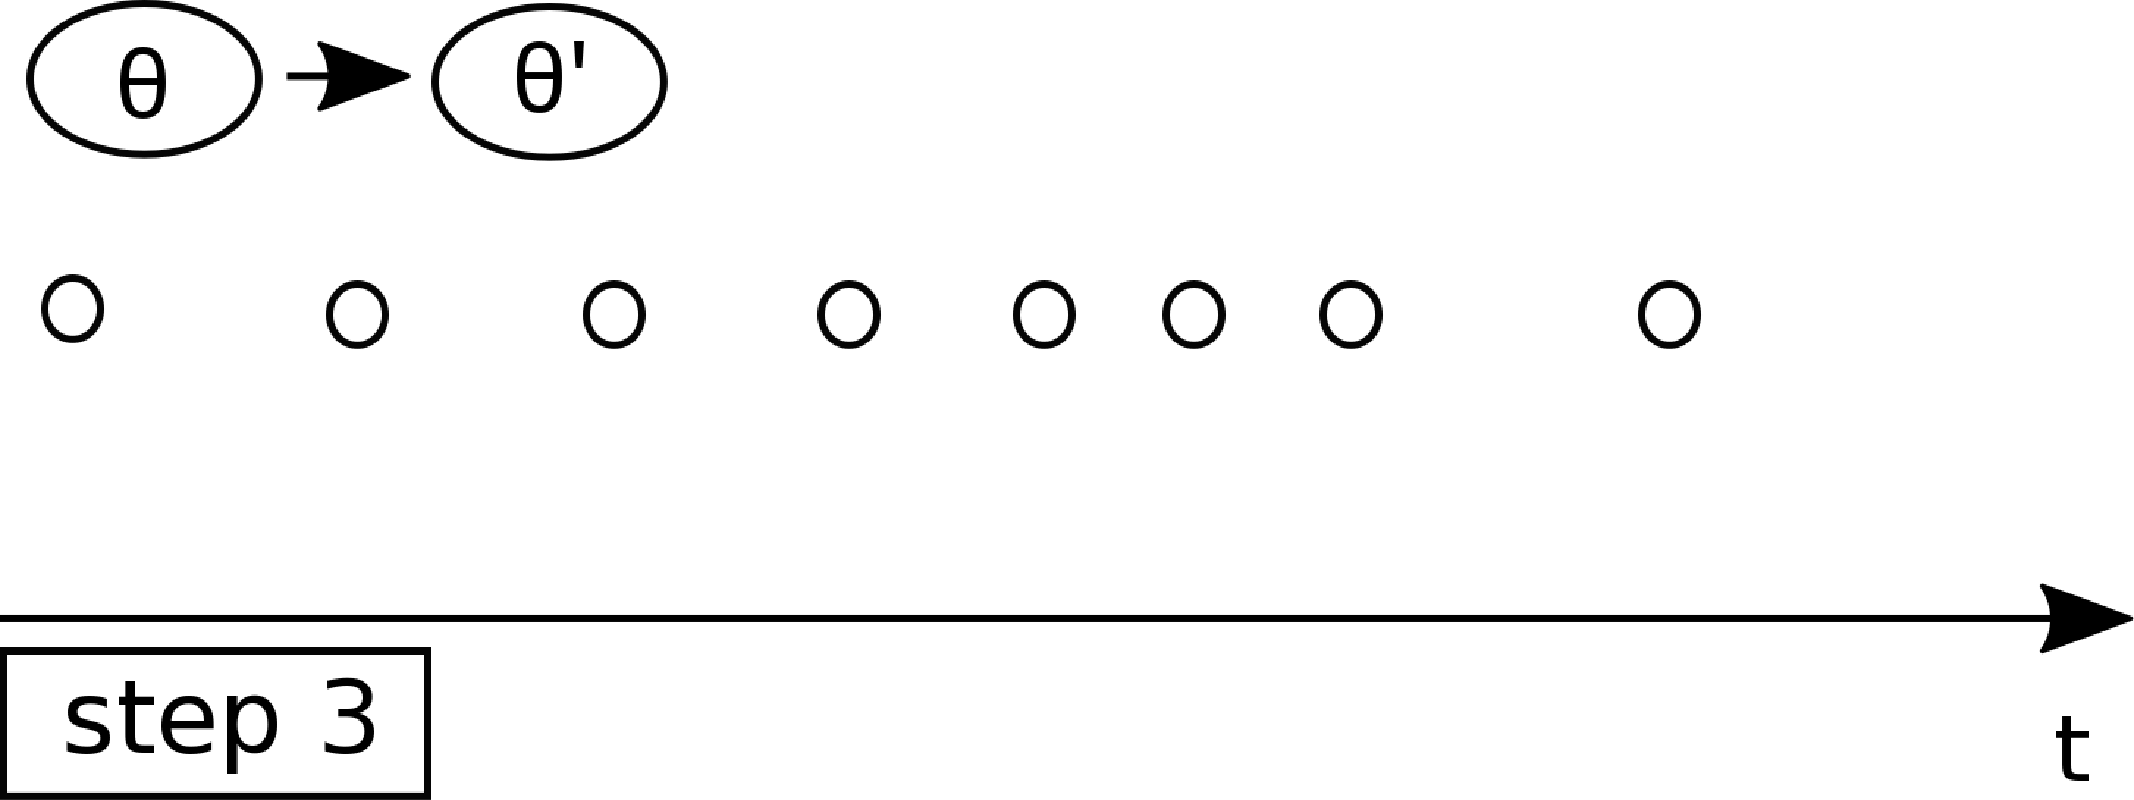
\includegraphics [width=0.96\textwidth, angle=0]{figs/plot3.png}
    \vspace{-0 in}
  \end{minipage}
% \begin{minipage}[hp]{0.45\linewidth}
% \centering
%   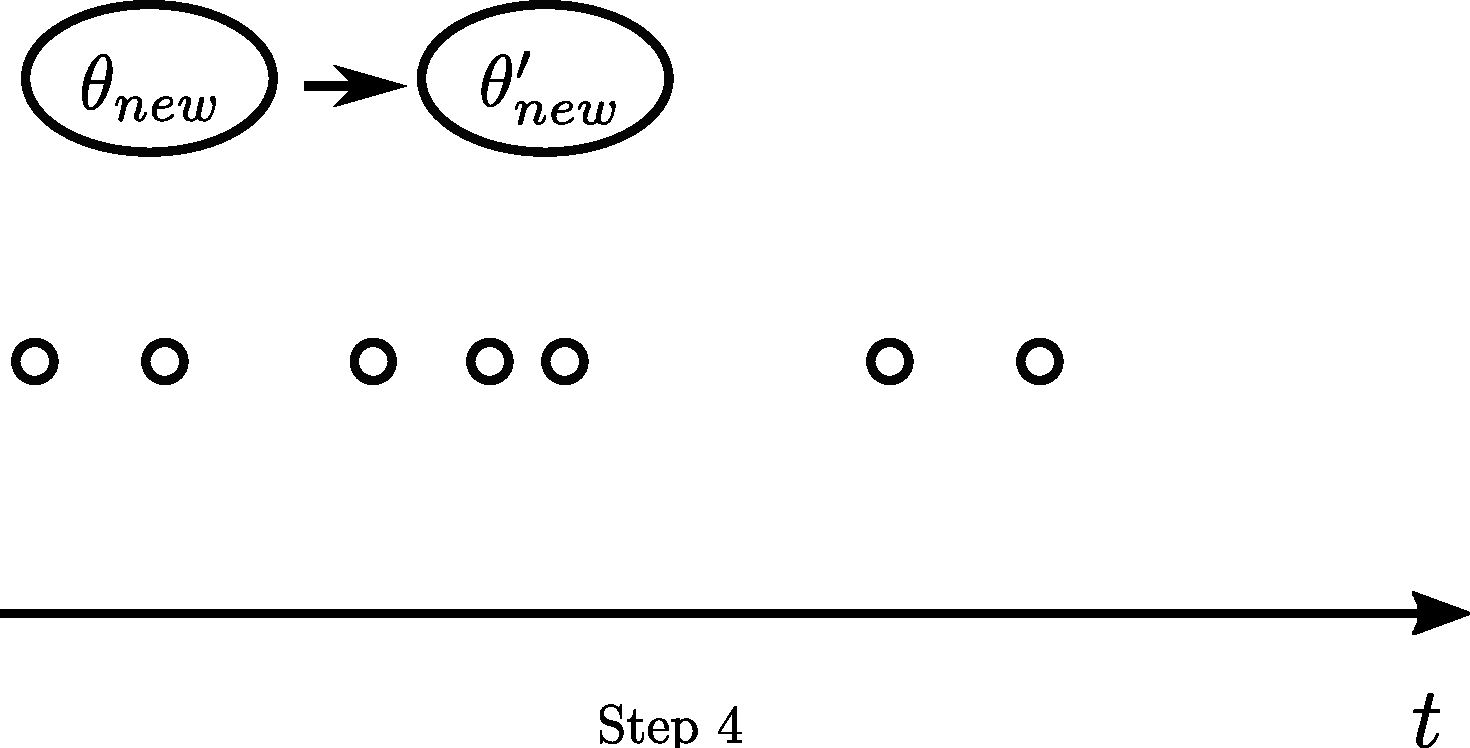
\includegraphics [width=0.70\textwidth, angle=0]{figs/plot4.pdf}
%   \vspace{-0 in}
% \end{minipage}
  \begin{minipage}[hp]{0.32\linewidth}
  \centering
    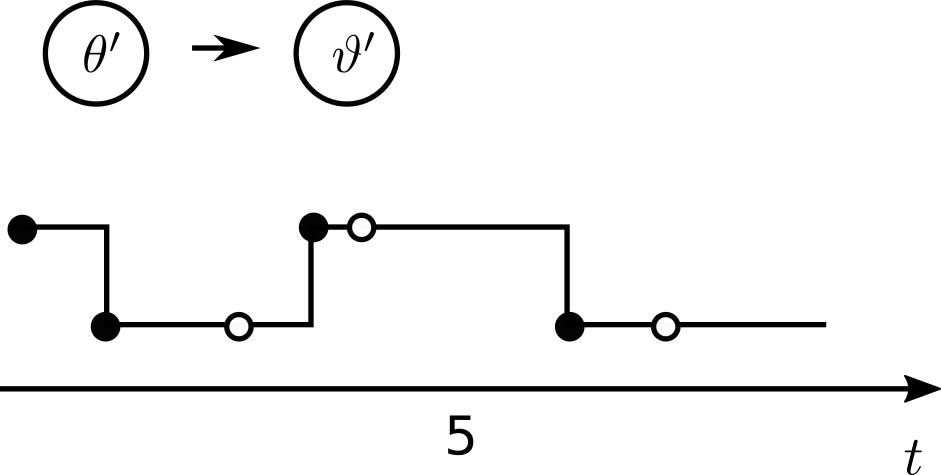
\includegraphics [width=0.96\textwidth, angle=0]{figs/plot5.png}
    \vspace{-0 in}
  \end{minipage}
  \begin{minipage}[hp]{0.32\linewidth}
  \centering
    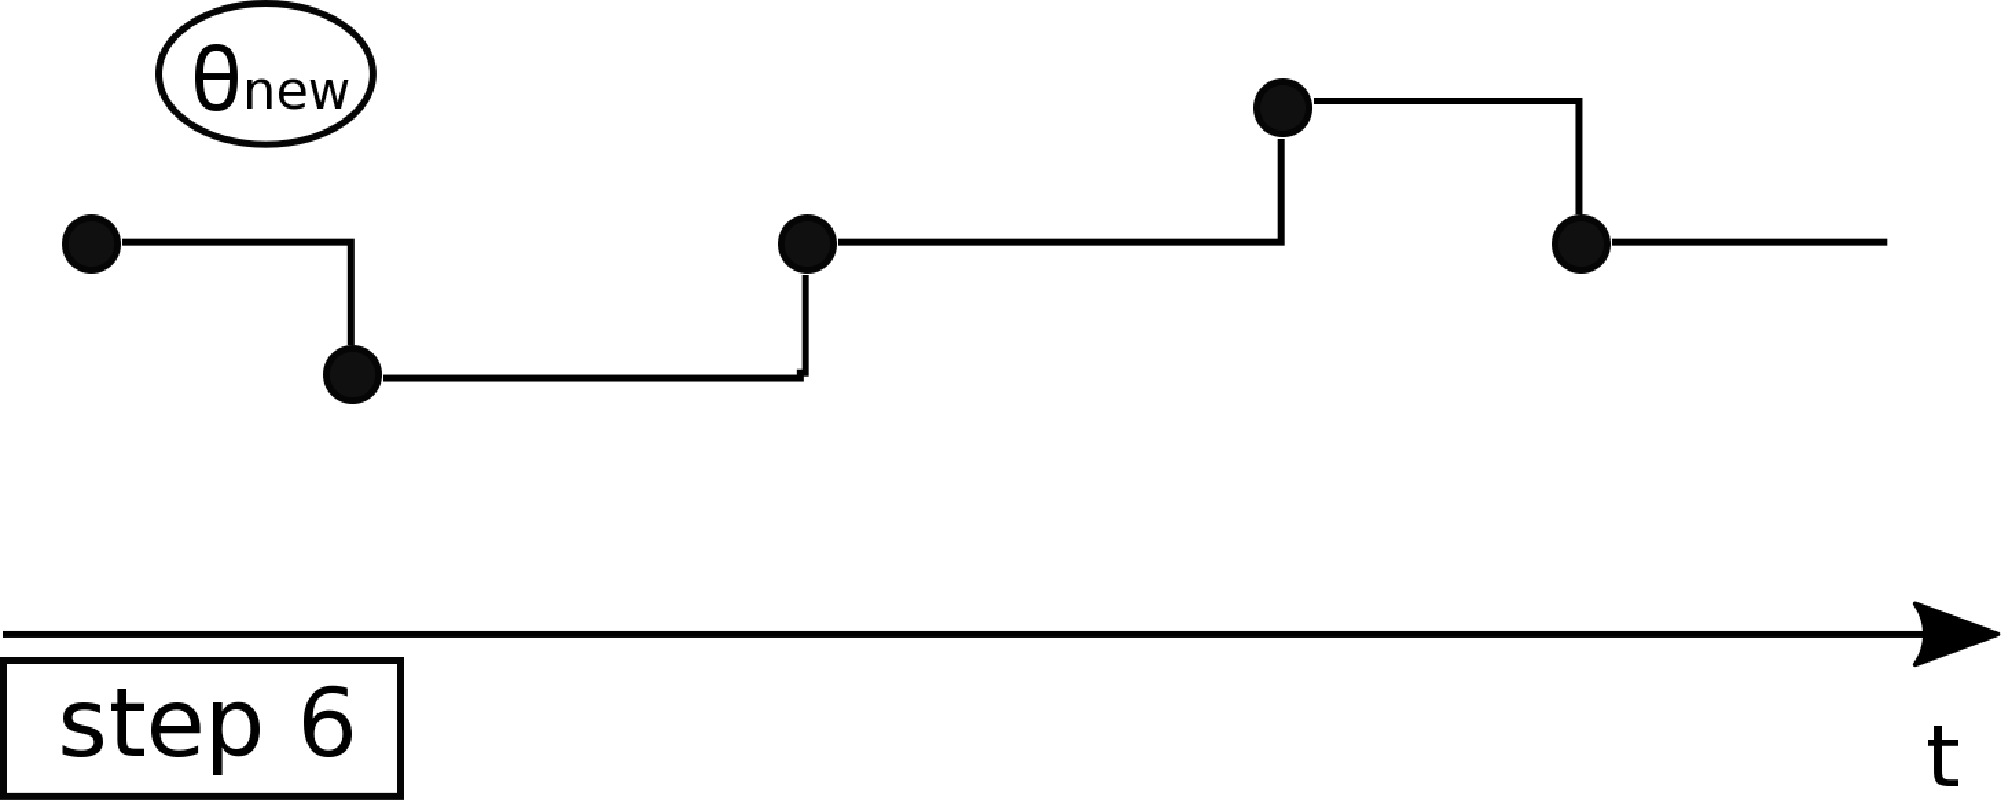
\includegraphics [width=0.96\textwidth, angle=0]{figs/plot6.png}
  \end{minipage}
    \caption{Symmetrized MH algorithm: Steps 1-3: Starting with a trajectory and parameter $\theta$, simulate an auxiliary parameter $\vartheta$, and then the thinned events
      $U$ from a rate $\Omega(\theta,\vartheta) - A_{S(\cdot)}$ Poisson
      process. Step 4: Discard state values, and propose swapping $\theta$ and $\vartheta$. Step 5:
      Run a forward pass to accept or reject this proposal, calling the new parameters $(\theta',\vartheta')$. 
    Use these to simulate a new trajectory. Step 6: Discard $\vartheta'$ and the thinned events.} 
   \label{fig:MH_improved}
  \end{figure}

